\section{Implementation}

\subsection{Transcription, RAG, and LLM Evaluation}
The backend is implemented as a FastAPI service and is organized around a small
set of domain-specific services. This design keeps the main AI workflow
separate from the user interface and makes each processing step easier to test
and inspect. The runtime pipeline begins with an audio recording of examiner
feedback. The transcription service sends this audio to the configured
KISSKI/SAIA speech endpoint and returns the transcribed text together with the
audio duration.

After transcription, the RAG pipeline prepares the text for evidence-grounded
evaluation. If required, the transcript is normalized into English so that
retrieval can work consistently across German and English inputs. The pipeline
then builds a criterion-aware retrieval query, retrieves relevant educational
evidence from the ChromaDB knowledge base, and applies filtering and quality
reranking to select the final evidence chunks. These chunks are not used as a
replacement for the transcript; rather, they provide educational guidance that
helps the LLM evaluate the feedback according to the defined rubric.

The knowledge base is prepared separately by the document-management service.
Source documents are parsed, split into semantically useful chunks, embedded
with the configured multilingual embedding model, and stored in ChromaDB. This
separation between offline knowledge-base preparation and online evaluation
makes the system easier to maintain. For example, a transcription failure,
retrieval problem, prompt issue, or JSON parsing error can be localized to a
specific service rather than being hidden inside one monolithic workflow.

The evaluation prompt combines three elements: the transcript, the retrieved
evidence, and the six-criterion feedback-quality rubric. It also defines the
expected response format. The LLM is asked to return a structured object
containing a short summary, criterion-level scores, suggestions, a key
suggestion, and optional quotes from the transcript. The backend then attaches
the transcript and duration, computes the overall score and the number of met
criteria, validates the result, and resolves it into German or English. This
structured response is important because it can be compared across RAG variants
and reused by the coaching endpoint. A purely free-form answer would be harder
to parse, evaluate, and connect to later system components.

The implementation also includes an interactive coaching step. Unlike the
initial evaluation prompt, the coaching prompt receives the previous evaluation,
the original transcript, the user's follow-up question, recent conversation
history, and retrieved evidence when relevant. This allows the system to explain
why a criterion received a certain score, suggest clearer feedback wording, or
connect an improvement suggestion to educational guidance. In this way, the
system moves beyond a one-time automated score and becomes a practice-oriented
feedback training tool.

\subsection{Model Configuration and Reproducibility}
The current system configuration uses:
\begin{itemize}
    \item evaluation model: \texttt{meta-llama-3.1-\allowbreak 8b-instruct};
    \item judge model: \texttt{gpt-oss-120b};
    \item embedding model: \texttt{multilingual-e5-large-instruct};
    \item transcription model: \texttt{whisper-large-v2}.
\end{itemize}

The current production RAG configuration follows the strongest variant observed
in the comparison workflow: \texttt{hyde\_k8}. Both evaluation and coaching
retrieval use HyDE-based retrieval with a candidate pool of 20, a final context
size of 8 chunks, English normalization enabled, criterion-aware query
construction enabled, and quality reranking enabled. In this setting, the pool
is split between direct retrieval from the transcript and retrieval from a
HyDE-generated hypothetical guidance passage. The resulting candidates are
deduplicated, reranked, filtered, and reduced to the final evidence context
passed into the LLM.

The RAG comparison outputs in the debug notebook were generated when the
evaluation model was configured as \texttt{llama-3.3-70b-instruct}. That model
is no longer supported in the current KISSKI setup, so the runtime evaluation
model was changed to \texttt{meta-llama-3.1-\allowbreak 8b-instruct}. The judge model
remains \texttt{gpt-oss-120b}, which is still the configured judge model.

This distinction matters for reproducibility. The notebook results should be
understood as an illustration of the retrieval design and comparison method
rather than a fully reproducible final benchmark under the current model
configuration. Future evaluation should repeat the comparison with the currently
available evaluation model and report whether the same retrieval ranking holds.

\subsection{Implementation Flowchart}
Figure~\ref{fig:implementation-flow} summarizes the implemented backend
workflow. The diagram separates the offline knowledge-base preparation from the
runtime examiner-feedback pipeline. This distinction is important because the
knowledge base can be updated independently, while the runtime path is executed
for each examiner feedback submission or coaching question.

\begin{figure}[p]
    \centering
    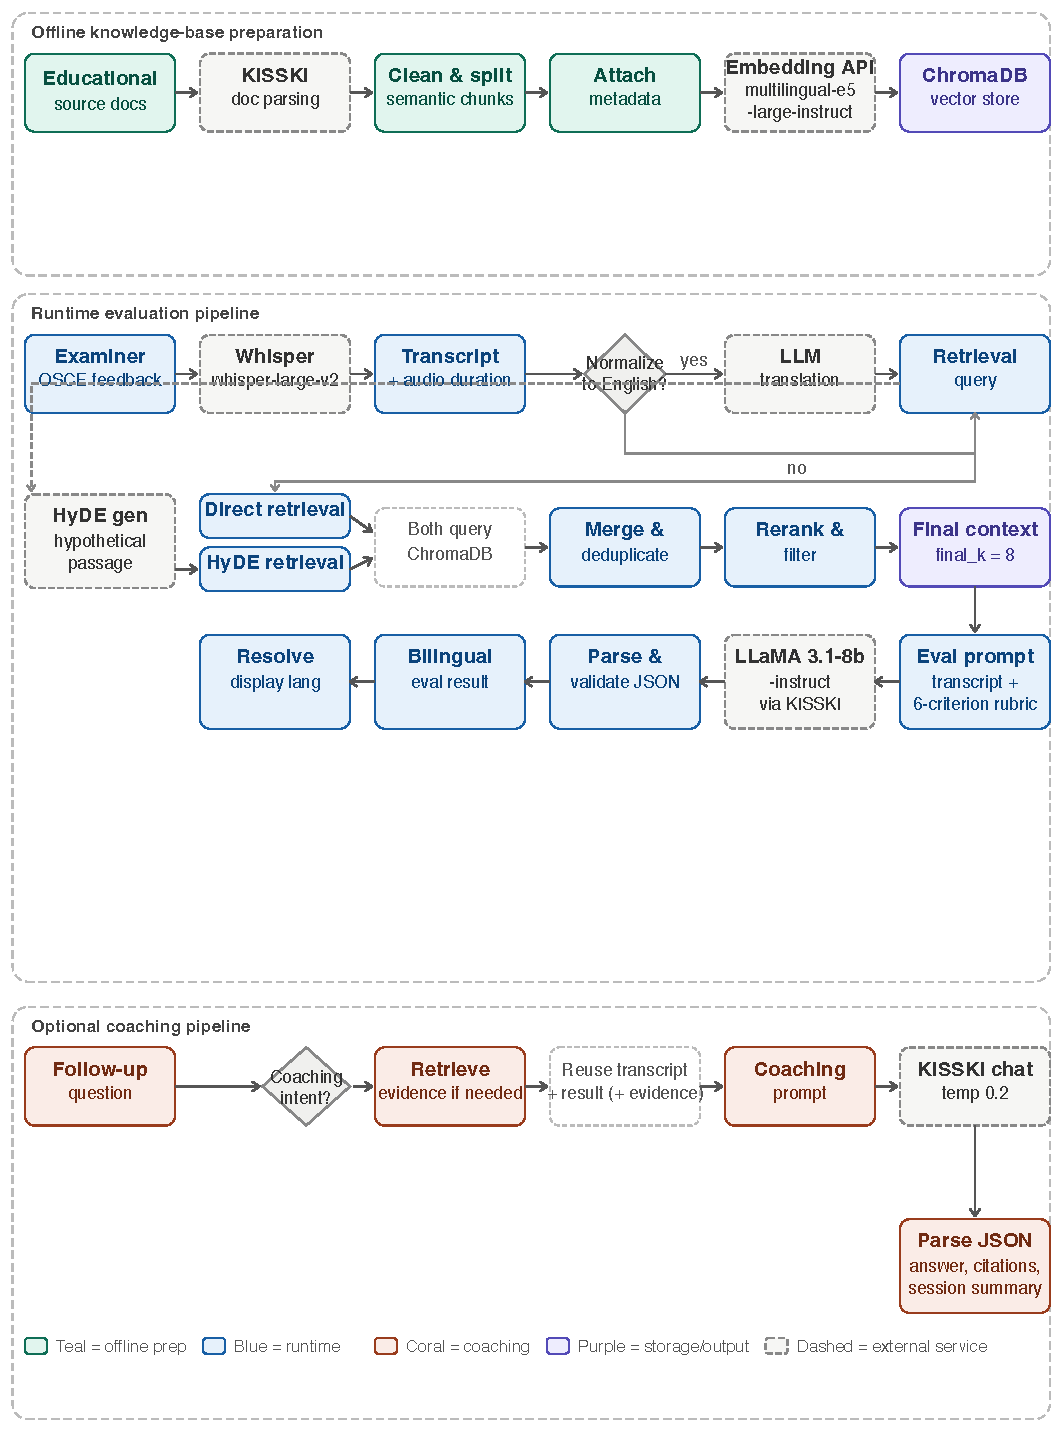
\includegraphics[width=\linewidth,height=0.78\textheight,keepaspectratio]{figures/examiner_coach_flow.pdf}
    \caption{Detailed implementation flow of Examiner Coach, including
    knowledge-base preparation, runtime evaluation, RAG retrieval, and optional
    coaching.}
    \label{fig:implementation-flow}
\end{figure}
